% !TEX encoding = UTF-8
% !TEX TS-program = pdflatex
% !TEX root = ../tesi.tex

%**************************************************************
\chapter{Valutazione retrospettiva e conclusioni}
\label{cap:conclusione}
%**************************************************************

\intro{In questo capitolo si andranno a presentare i possibili sviluppi di questo progetto in base ai risultati ottenuti.}

\section{Migliorie software}
Si riportano qui alcune attività da svolgere per far evolvere la Proof of Concept ad un applicativo più completo.

\subsection{Classificazione oggetti tramite machine learning}
Alla fine del periodo di tirocinio, il software prodotto per la Proof of Concept indica una piena fattibilità del progetto. In particolare l'analisi del modello di machine learning realizzato dice che la classificazione di oggetti tramite la firma spettrale produce risultati accettabili. Una possibile difficoltà che l'azienda potrà incontrare nel caso decidesse di portare avanti il progetto sarà l'individuazione di un dataset adatto per allenare la rete neurale. Infatti il committente richiede che il software sia in grado di riconoscere eventuali malattie delle colture ed il grado di maturazione. Con il dataset di USGS questo compito non è implementabile, sarà quindi necessario individuarne uno adatto tramite una ricerca più approfondita oppure crearne uno. Per la seconda opzione sarà necessario investire molte risorse aziendali, in modo da acquisire molte rilevazioni delle colture che si vorranno analizzare in diverse condizioni, quindi il tempo necessario alla raccolta dei dati sarà molto lungo.

\subsection{Esposizione modello allenato}
Un'altra decisione da prendere sarà se condividere il modello di machine learning tra le varie istanze dell'applicazione oppure no. Nel primo caso sarà bene migrare verso un'infrastruttura cloud che offra servizi di machine learning integrati, in modo da garantire scalabilità e performance elevate. Infatti con l'architettura client-server attuale è possibile soltanto scalare verticalmente le risorse, cosa alquanto limitante.

\subsection{Business logic}
L'algoritmo proposto durante il tirocinio per il calcolo del percorso è euristico. Con più tempo a disposizione sarà bene analizzarne le prestazioni in applicazioni reali (anche simulate) e, se necessario, pensare ed implementare una soluzione più efficiente. Inoltre allo stato attuale è previsto al massimo un drone per ogni campo di colture, potrebbe essere interessante sviluppare un algoritmo per più droni in caso di campi molto estesi, visto che molto probabilmente la batteria del singolo potrebbe non essere sufficiente a svolgere un'analisi completa in un solo volo.

\section{Valutazione retrospettiva personale}
La pianificazione delle attività svolta a monte dell'inizio del tirocinio ha subito molte variazioni per via del carattere sperimentale del progetto. Tuttavia una volta identificati i punti cardine, ovvero nella seconda settimana, si è definita in modo stabile la collocazione temporale delle attività da svolgere. Il carico di lavoro risultante è stato adeguato al tempo a disposizione, riuscendo a rimanere in pari con quanto preventivato. Tutti gli obiettivi presentati nella sezione \ref{sec:pianificazione} sono stati raggiunti durante lo svolgimento dello stage.

\section{Riassunto quantitativo impegno orario}
Viene riportato in figura \ref{fig:impegno_orario} un istogramma con il numero di ore impiegato per ogni attività svolta durante il periodo di tirocinio. L'attività di analisi del problema include anche le ore impiegate nella ricerca di un dataset adatto, visto che la definizione della rappresentazione di un singolo esempio era fortemente legata al tipo di dati trovati in rete. Da questo si evince che una parte consistente del tirocinio è stata dedicata all'analisi prestazionale di vari modelli di machine learning, oltre che al tempo necessario per apprendere la teoria alla base e fare quindi considerazioni utili.

\begin{figure}
    \centering
    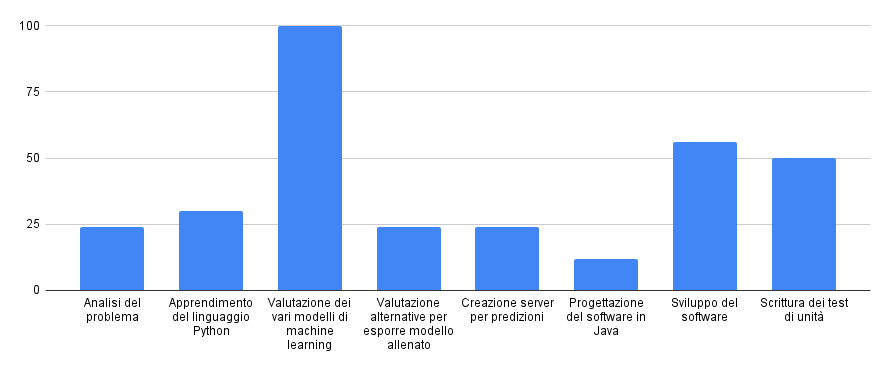
\includegraphics[width=\textwidth]{immagini/impegno_orario.png}
    \caption{Istogramma impegno orario per attività}
    \label{fig:impegno_orario}
\end{figure}
